% chktex-file 13 chktex-file 26
%%%%%%%%%%%%%%%%%%%%%%%%%%%%%%%%%%%%%%%%%
% Stylish Article
% LaTeX Template
% Version 2.1 (1/10/15)
%
% This template has been downloaded from:
% http://www.LaTeXTemplates.com
%
% Original author:
% Mathias Legrand (legrand.mathias@gmail.com) 
% With extensive modifications by:
% Vel (vel@latextemplates.com)
%
% License:
% CC BY-NC-SA 3.0 (http://creativecommons.org/licenses/by-nc-sa/3.0/)
%
%%%%%%%%%%%%%%%%%%%%%%%%%%%%%%%%%%%%%%%%%

%----------------------------------------------------------------------------------------
%	PACKAGES AND OTHER DOCUMENT CONFIGURATIONS
%----------------------------------------------------------------------------------------

\documentclass[fleqn,10pt]{SelfArx} % Document font size and equations flushed left

\usepackage[ngerman]{babel} % Specify a different language here - english by default
\usepackage{csquotes}

\usepackage{listings}

\usepackage{biblatex} 
\usepackage{indentfirst}
\addbibresource{literatur.bib}

%----------------------------------------------------------------------------------------
%	COLUMNS
%----------------------------------------------------------------------------------------

\setlength{\columnsep}{0.55cm} % Distance between the two columns of text
\setlength{\fboxrule}{0.75pt} % Width of the border around the abstract

%----------------------------------------------------------------------------------------
%	COLORS
%----------------------------------------------------------------------------------------

\definecolor{color1}{RGB}{0,0,90} % Color of the article title and sections
\definecolor{color2}{RGB}{0,20,20} % Color of the boxes behind the abstract and headings

%----------------------------------------------------------------------------------------
%	HYPERLINKS
%----------------------------------------------------------------------------------------

\usepackage{hyperref} % Required for hyperlinks
\hypersetup{hidelinks,colorlinks,breaklinks=true,urlcolor=color2,citecolor=color1,linkcolor=color1,bookmarksopen=false,pdftitle={Title},pdfauthor={Author}}

%----------------------------------------------------------------------------------------
%	ARTICLE INFORMATION
%----------------------------------------------------------------------------------------

\JournalInfo{Handout, \today} % Journal information
\Archive{Dieses Werk ist unter einer Creative Commons Lizenz vom Typ Namensnennung 2.0 Deutschland zugänglich. Um eine Kopie dieser Lizenz einzusehen, konsultieren Sie http://creativecommons.org/licenses/by/2.0/de/ oder wenden Sie sich brieflich an Creative Commons, Postfach 1866, Mountain View, California, 94042, USA.} % Additional notes (e.g. copyright, DOI, review/research article)

\PaperTitle{Web-Dashboard} % Article title

\Authors{Marvin Gaube\textsuperscript{1}, Sidney Kuyateh\textsuperscript{1}, Steffen Walter\textsuperscript{1}} % Authors
\affiliation{\textsuperscript{1}\textit{Studiengang Informationstechnik, Fakultät Technik, Duale Schule Baden-Württemberg, Stuttgart}} % Author affiliation


\Keywords{} % Keywords - if you don't want any simply remove all the text between the curly brackets
\newcommand{\keywordname}{Keywords} % Defines the keywords heading name

%----------------------------------------------------------------------------------------
%	ABSTRACT
%----------------------------------------------------------------------------------------

\Abstract{Die vorliegende Dokumentation gibt einen kurzen Einblick in das Projekt \enquote{Web-Dashboard} geben, und dabei insbesondere auf folgende Architekturelemente eingehen:
\begin{itemize}
    \item Allgemeine Struktur
    \item Anbindung der Openweathermap-API
    \item Anbindung der Wikipedia-API und der Watson TTS-API
    \item Einbindung eines RSS-Feeds
    \item Einbindung eines Mastodon-Feeds inklusive Authentifizierung ggü.\ der Mastodon-Instanz
    \item Einbindung der VVS-API
\end{itemize}
}

%----------------------------------------------------------------------------------------

\begin{document}

\flushbottom % Makes all text pages the same height

\maketitle % Print the title and abstract box

\tableofcontents % Print the contents section

\thispagestyle{empty} % Removes page numbering from the first page

%----------------------------------------------------------------------------------------
%	ARTICLE CONTENTS
%----------------------------------------------------------------------------------------

\section*{Einleitung} % The \section*{} command stops section numbering

\addcontentsline{toc}{section}{Einleitung} % Adds this section to the table of contents
Aufgabenstellung war, mittels Webtechnologien ein Portal zu entwickeln, dass einige dynamische/interaktive Funktionalitäten --- insbesondere unter Einbindung externer Schnittstellen --- mit einbindet. 

%------------------------------------------------
\section{Grundlegende Architektur}
Das Projekt ist in zwei Module aufgeteilt: \textbf{Frontend} und \textbf{Backend}.

Das Frontend ist mit HTML, CSS und JavaScript realisiert und läuft komplett Clientseitig, also im Browser. Teilweise kommt das Framework \enquote{Vue}~\cite{vue} zum Einsatz.

Das Backend ist ebenfalls in JavaScript mithilfe der Laufzeitumgebung Node.js~\cite{nodejs} realisiert und übernimmt die Auslieferung des Frontends sowie Authentifizierungs- und Proxyaufgaben. Für die HTTP-Schnittstelle kommt das Node-Modul Express~\cite{express} zum Einsatz.
\section{Aufbau der Oberfläche}

\section{Backend}
Das Backend ist mittels express.js~\cite{express} aufgebaut. Für die Authentifizierung gegenüber Mastodon-Instanzen kommt noch eine Dateibasierte SQLITE-Datenbank mit der Abstraktionsschicht \enquote{Sequelize}~\cite{sequelize} zum Einsatz, die Applikations-ID und Secret speichert. Weiterhin ist der HTTP-POST-Endpunkt \enquote{/getTTS} vorhanden, der einen Proxy zur IBM-Watson-TTS-API bildet und die Authentifizierung übernimmt. \\
Ein simpler Proxy - /getFile" - ist für die Überwindung der CORS-Problematik beim Nachladen externer Ressourcen notwendig. \\
Die Konfiguration --- insbesondere die der API-Schlüssel --- erfolgt über Umgebungsvariablen, die mittels dem Modul \enquote{dotenv}~\cite{dotenv} aus der lokalen Datei \texttt{.env} geladen werden. Damit wird eine Trennung von Code/Applikation und Konfigurationsdaten erreicht --- eine Beispieldatei für \texttt{.env} (\texttt{.exampleenv}) ist jedoch weiterhin vorhanden. \\
\section{Integration von Mastodon}
Mastodon ist ein Twitterähnliches, verteiltes soziales Netzwerk. Verteilt bedeutet, dass es beliebig viele Instanzen gibt, deren Nutzer über das sogenannte \enquote{ActivityPub}-Protocol miteinander interagieren können. Ziel der Implementierung ist es, dem Nutzer seine persönliche Timeline (die letzten Posts) in einer Kachel anzuzeigen.
\subsection{Authentifizierung}
Um die nichtöffentlichen Teile der Mastodon-REST-API nutzen zu können, muss sich der Nutzer dem Server gegenüber authentifizieren. Eine zusätzliche Schwierigkeit ist, dass dies nicht gegenüber einem festen Endpunkt erfolgt, sondern davon abhängt, bei welchem Server (auch: Instanz) der Nutzer registriert ist. Beispiele für solche Instanzen sind \enquote{chaos.social} und \enquote{mastodon.social}. \\
Der grundlegende Ablauf ist hierbei in Bild~\ref{fig:mastodon1} zu sehen. Jede Applikation bekommt von der Mastodon-Instanz eine ID und ein Secret, welches vom Backend automatisch bezogen und gespeichert wird. Hierbei unterstützt das Backend beliebig viele Instanzen, es kommt eine sqlite-Datenbank zum Einsatz (siehe: backend/models/appData.js).

Der Client leitet mit Kenntnis der App-ID zur Authentifizierungsseite weiter, bei der der Nutzer unserer App Rechte vergeben oder ablehnen kann. Zurück kommt ein Code, mit dem das Backend (unter Zuhilfenahme des secrets und der ID) einen Token abholen kann. Dieser wird im Browser lokal als Cookie gespeichert.
\subsection{Anzeige der Timeline}
Das Frontend führt nach der Authentifizierung alle Kommunikation mit dem Mastodon-Server selbstständig durch. Hierzu wird, entweder das Formular zur Authentifizierung angezeigt, oder per REST die Posts aus der Timeline abgeholt. Diese werden dann, in ein HTML gerendert, in die Kachel geschrieben. Es kommt die fetch-API für HTTP-Anfragen zum Einsatz.

Die Funktion ist in Bild~\ref{fig:demo1},~\ref{fig:demo2} und~\ref{fig:demo3} zu sehen. Die Implementierung erfolgt in der \enquote{\texttt{mastodon.mjs}}.

\section{Kurzanleitung}
Um die Software zu erhalten müssen zuerst die beiden Git Repositories für das Frontend und das Backend heruntergeladen werden. Dies kann zum Beispiel durch den diese Befehle erfolgen:
\begin{lstlisting}
git clone https://github.com/activityp
  ub-frontend/backend.git
git submodule update --init --recursive
\end{lstlisting}
Mit dem zweiten Befehl wird das Frontend Repository in den gewünschten Ordner im Backend platziert.
Um alle nötigen Abhängigkeiten herunter zu laden muss folgendes Kommando im Wurzelverzeichnis des Backend Ordners ausgeführt werden:
\begin{lstlisting}
npm install
\end{lstlisting}
Als nächstes muss die die Datei .exampleenv in .env umbenannt werden und es müssen die entsprechenden API Token und Zugangsdaten eingegeben werden um die externen Dienste ansprechen zu können.
Mit einem der Folgenden Kommandos kann dann das Backend gestartet werden:
\begin{lstlisting}
npm run debug
node server.js
\end{lstlisting}
Nun ist der Server unter localhost auf Port 5000 erreichbar und das Frontend kann intuitiv bedient werden.  \\
Die Mastodon-Einbindung funktioniert  nur, wenn man das Dashboard über dashboard.tinf17.in aufruft, da in der App-Anmeldung eine Weiterleitung nötig ist. Zum Test ist ein Account bei einem beliebigen Mastodon-Netzwerk, z.B. mastodon.social, notwendig.
\section{Fazit}
Das vorliegende Projekt hat uns sowohl auf inhaltlicher als auch auf persönlicher Ebene weiter gebracht und wir konnten unsere Erfahrungen im Bereich Webtechnologien stark ausbauen.
\subsection{Projektverlauf}
Das Projekt lief neben einigen wenigen Stolpersteinen ohne größere Hindernisse ab. Wie bei den meisten Gruppenarbeiten war es auch bei dieser nicht immer leicht, eine faire Aufteilung der Arbeitspakete zu gewährleisten. Für die Zukunft nehmen wir mit, dass wir zu einem früheren Zeitpunkt Methoden aus dem Projektmanagement einsetzen wollen, um einen reibungslosen Ablauf, faire Arbeitsteilung und die Vermeidung von doppelter Arbeit zu gewährleisten.
\subsection{Technologien}
Vor allem die Arbeit mit dem JavaScript-Framework \enquote{Vue}~\cite{vue} war für uns alle neu. Das Framework hat uns aber durch den geringen Overhead und die einfache Handhabe sehr überzeugt. Die Arbeit mit \enquote{Vue} hat uns weitergebracht und uns einen neuen Horizont in der Webentwicklung eröffnet. 
Auch war die Arbeit mit der Mastodon API neu und CSS wurde auch noch von keinem von uns in der Tiefe wie in diesem Projekt verwendet. Alles in allem kann gesagt werden, dass wir einige neue Technologien lernen und schätzen gelernt haben und einige Alte noch besser verstanden haben.
\subsection{Schwierigkeiten und Komplexität}
Wirkliche Schwierigkeiten gab es bei der Implementierung nicht. Zu beachten ist natürlich, dass man durch Authentifizierung viel mehr Datenflüsse und auch Zustände hat, als es in einem reinen REST-API-Aufruf der Fall wäre. Insbesondere die Einbindung des Backends ist hier zu erwähnen, da Secrets auf keinen Fall zum Client gelangen dürfen.
\begin{figure*}
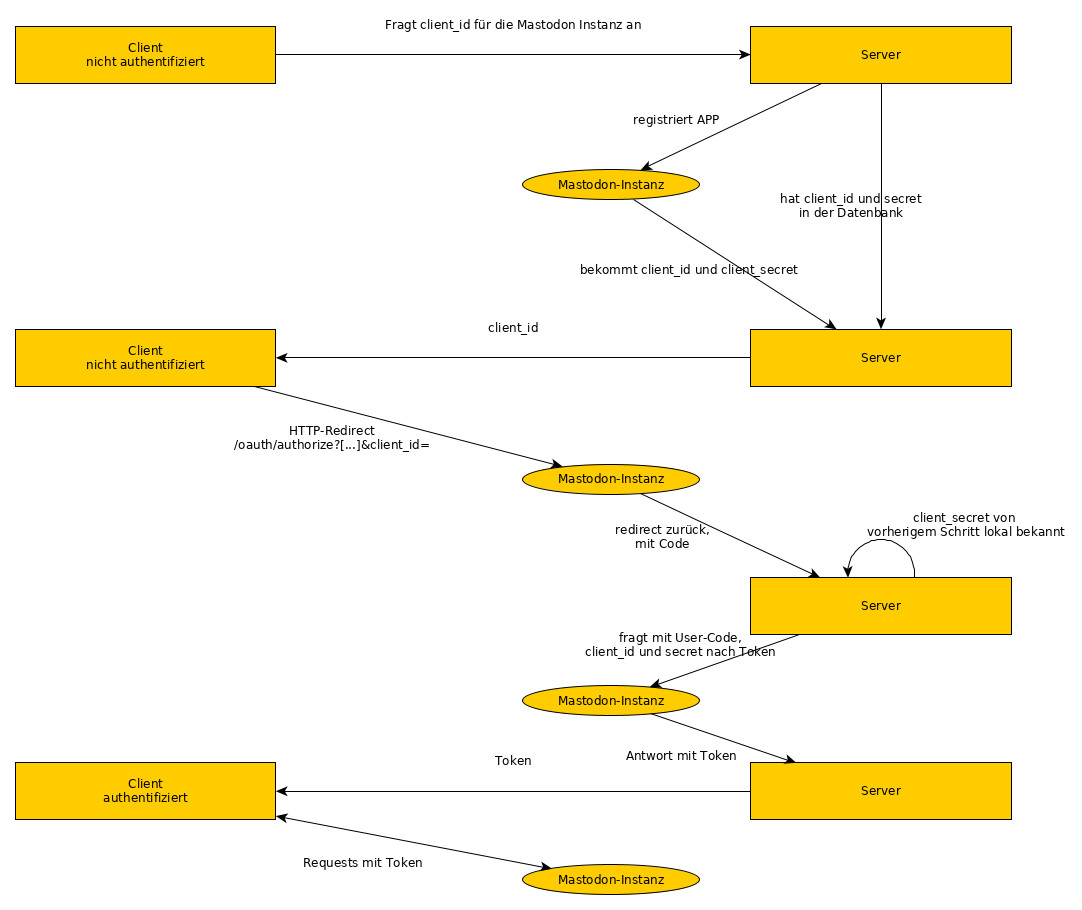
\includegraphics[width=\linewidth]{mastodon.jpg}
\caption{Mastodon Authentication}\label{fig:mastodon1}
\end{figure*}
\begin{figure*}
    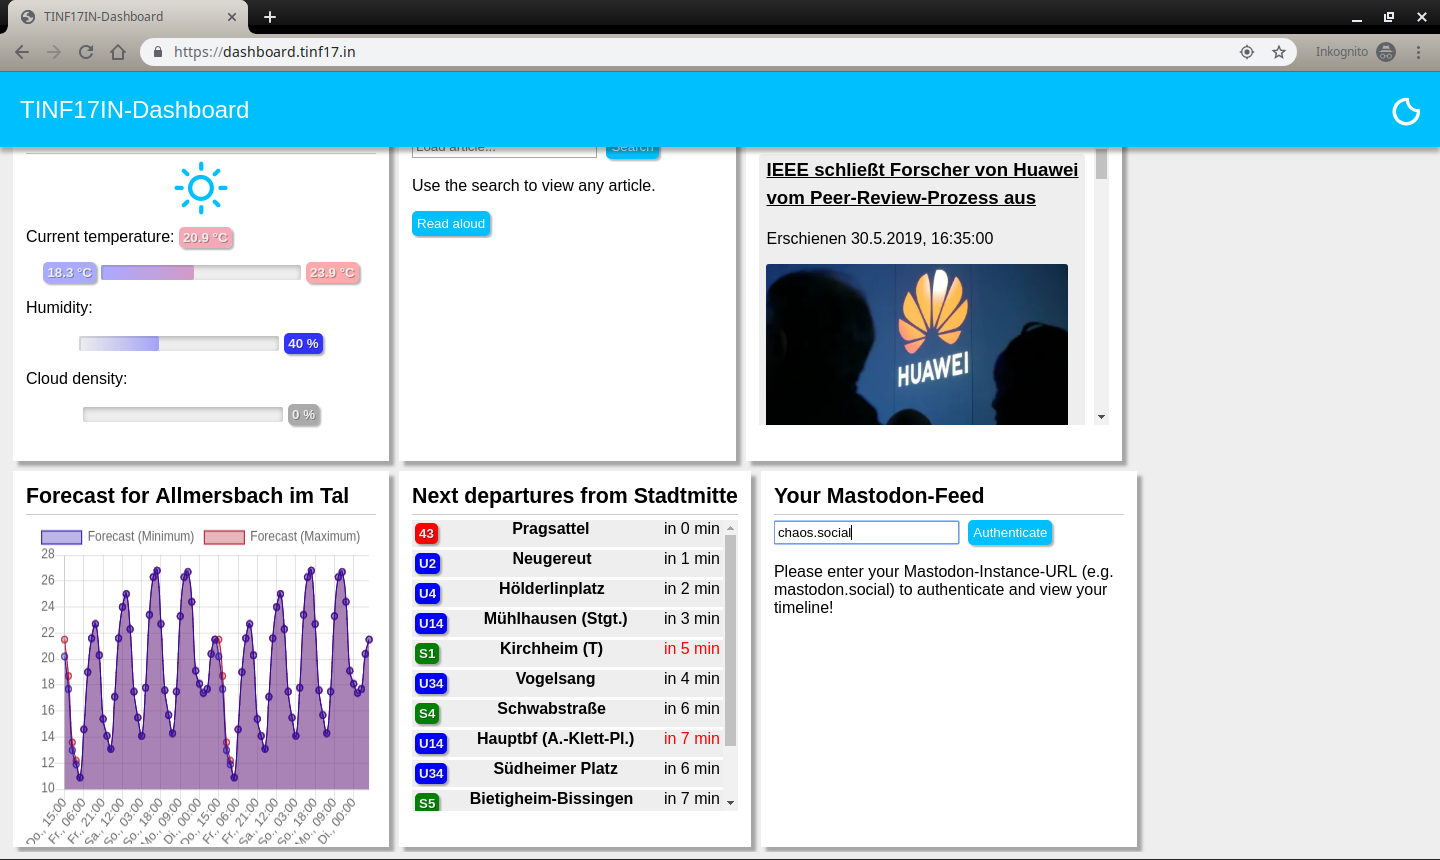
\includegraphics[width=\linewidth]{images/1.png}
    \caption{Dashboard mit inaktivem Mastodon}\label{fig:demo1}
\end{figure*}
\begin{figure*}
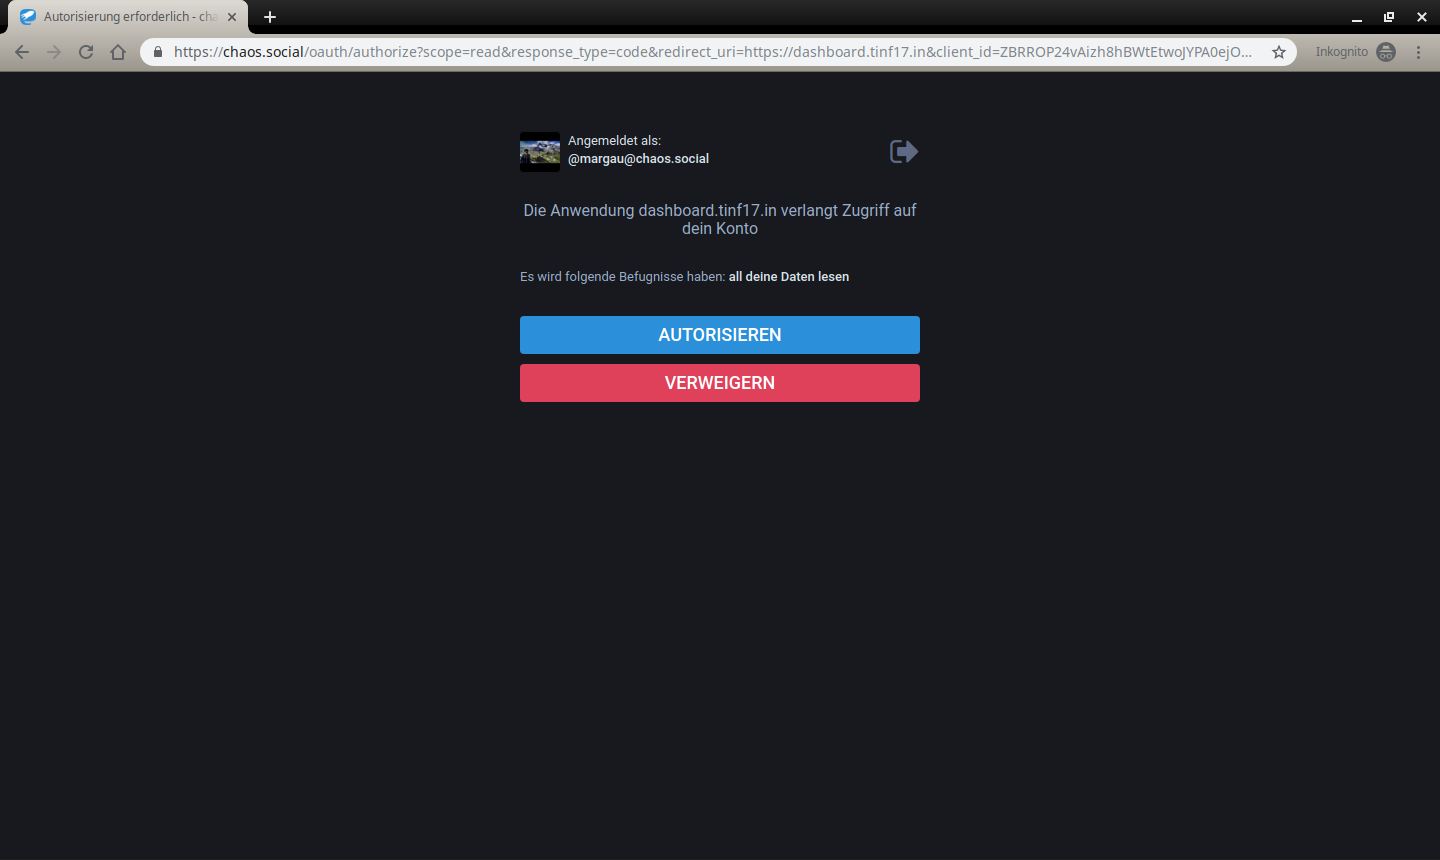
\includegraphics[width=\linewidth]{images/2.png}
\caption{Mastodon Authentifizierung bei chaos.social}\label{fig:demo2}
\end{figure*}

\begin{figure*}
    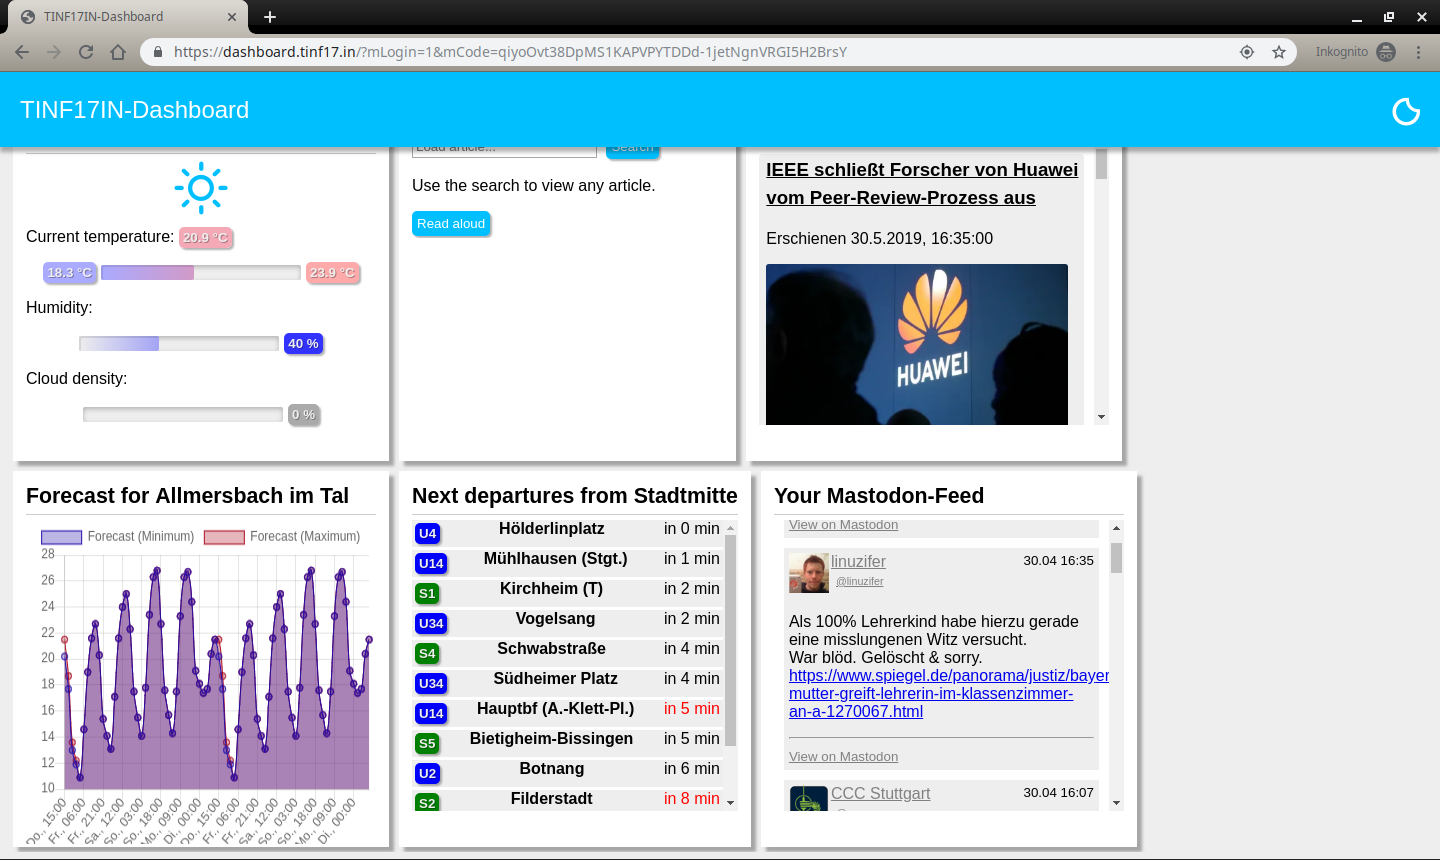
\includegraphics[width=\linewidth]{images/3.png}
    \caption{Demo, Mastodon aktiv}\label{fig:demo3}
\end{figure*}
\begin{figure*}
	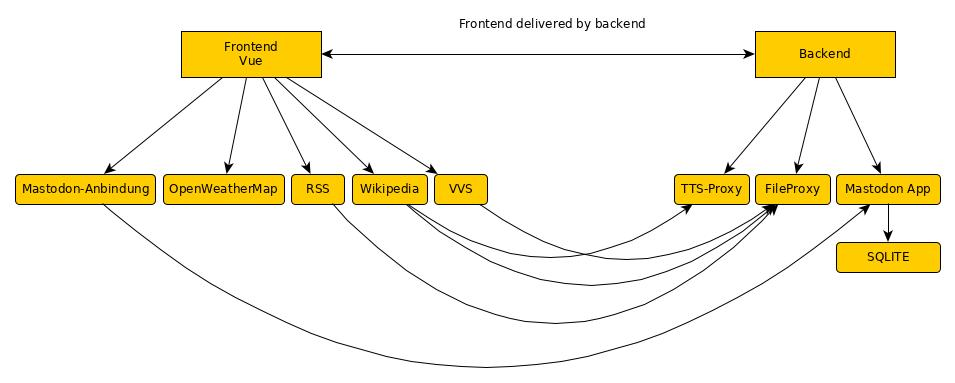
\includegraphics[width=\linewidth]{systemcomponent.jpg}
	\caption{Überblick über die Komponenten}
	\label{fig:component}
\end{figure*}


%\begin{figure}[ht]\centering % Using \begin{figure*} makes the figure take up the entire width of the page
%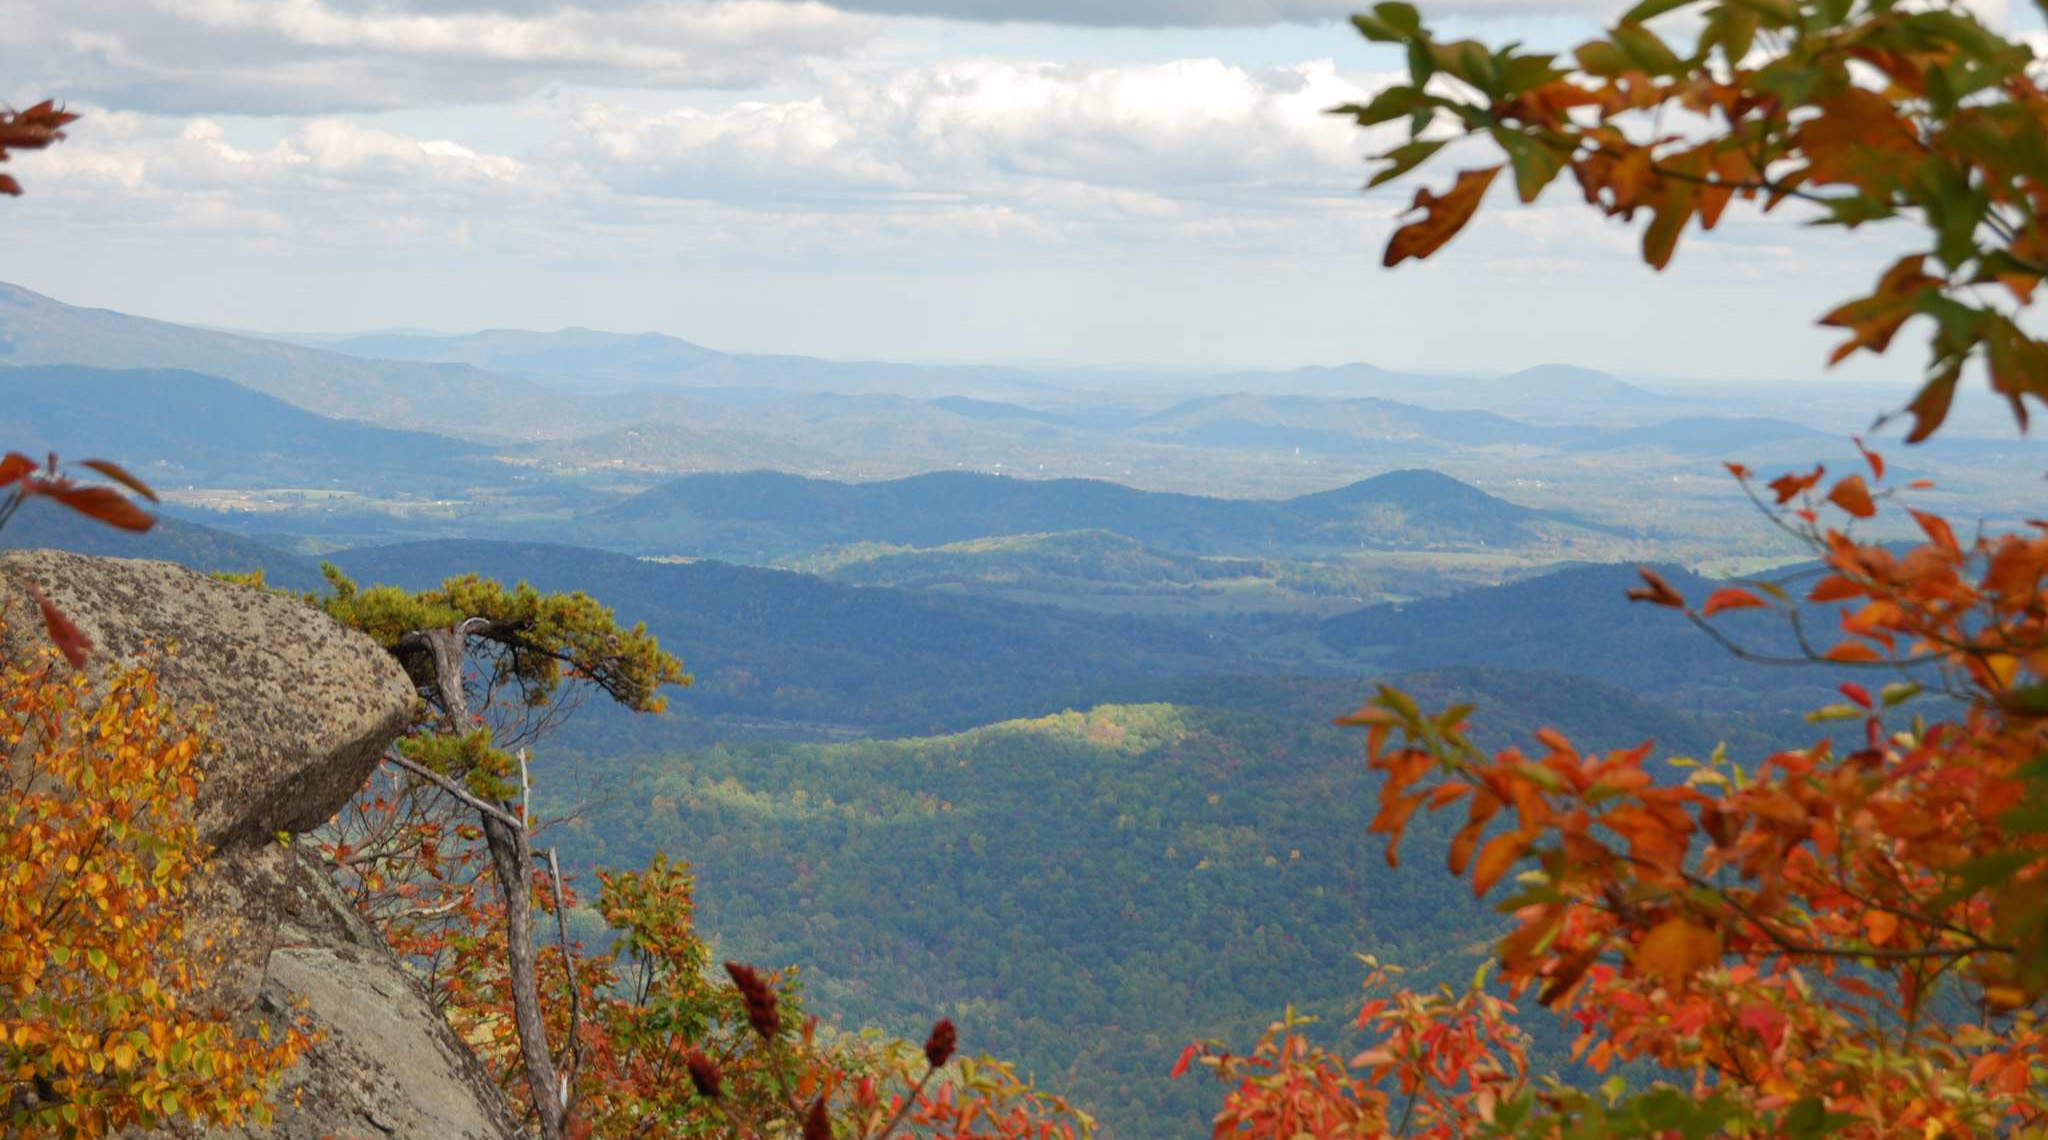
\includegraphics[width=\linewidth]{view}
%\caption{Wide Picture}
%\label{fig:view}
%\end{figure*}


%------------------------------------------------

%----------------------------------------------------------------------------------------
%	REFERENCE LIST
%----------------------------------------------------------------------------------------
%\phantomsection%
\printbibliography%
\end{document}